%\usepackage{wx672cjk}

\addbibresource{os.bib}

\begin{document}

\mode<article>{
  \title{C Programming under Linux}
  \subtitle{Lecture Handouts}
  \author{WANG Xiaolin\\{\small \url{wx672ster@gmail.com}}}
  \maketitle
  \tableofcontents
  \listoffixmes
%  \printbibliography[title={References}]{}
}

\begin{frame}<beamer>
  \title{C Programming under Linux}
  \author{WANG Xiaolin\\{\small \url{wx672ster@gmail.com}}}
  \titlepage
\end{frame}

\begin{frame}{References}
  \begin{small}
    \begin{refsection}
      \nocite{stevens2013advanced, raymond2003art, matthew2008beginning, kernighan2006c,
        king2008c, reek1997pointers, weiss1993data, waite1987c}
      \printbibliography[heading=none]
    \end{refsection}
  \end{small}
\end{frame}

\section{Introduction}

\begin{frame}{Program Languages}
  \begin{block}{Machine code}
    The \alert{binary numbers} that the CPUs can understand.
    \begin{center}{\ttfamily
      100111000011101111001111 ... and so on ...}
    \end{center}
  \end{block}
  \begin{block}{Assembly language --- friendly to humans}
    People don't think in numbers.
    \begin{center}
      \mode<beamer>{ \includegraphics[width=.5\textwidth]{asm-sample-asm} }%
    \end{center}
    \mode<article>{ \includegraphics[width=.2\textwidth]{asm-sample-asm} }
    The ASM programs are translated to machine code by \alert{assemblers}.
  \end{block}
\end{frame}

\begin{frame}
  \begin{block}{High level languages}
    Even easier to understand for humans. Examples:
    \begin{itemize}
    \item C\tikzmark{clang}
    \item FORTRAN\tikzmark{fortran}
    \item Java\tikzmark{java}
    \item C++\tikzmark{cpp}
    \item ...\tikzmark{more}
    \end{itemize}\pause
    \alert{Compilers} do the translation work.    
  \end{block}
  \begin{tikzpicture}[remember picture,overlay,
    every node/.style={ellipse,red,opacity=.4,draw},
    every to/.style={append after command={[->,black!30,thick]}}
    ]
    \node (asm) at ($(pic cs:java) + (3,0)$) {Assembly};
    \node (bin) [right=of asm] {Binary};
    \draw ($(pic cs:clang)+(0,.5ex)$) to [bend left=20] (asm);
    \draw ($(pic cs:fortran)+(0,.5ex)$) to [bend left=15] (asm);
    \draw ($(pic cs:java)+(0,.5ex)$) to (asm);
    \draw ($(pic cs:cpp)+(0,.5ex)$) to [bend right=15] (asm);
    \draw ($(pic cs:more)+(0,.5ex)$) to [bend right=20] (asm);
    \draw (asm) to (bin);
    \end{tikzpicture}
\end{frame}

\begin{frame}{The History of C}
  \begin{description}
  \item[1967] \alert{BCPL} (Basic Computer Programming Language), Martin Richards
  \item[1970] \alert{B}, Bell Labs, Ken Thompson
  \item[1970+] \alert{C}, Bell Labs, Dennis Ritchie
  \item[1978] \alert{The C Programming Language}, B.Kernighan/D.Ritchie
  \item[1980] \alert{C++}, Bjarne Stroustrup
  \item[1989] \alert{ANSI C}, American National Standards Institute
  \item[1999] \alert{ISO/IEC 9899 C}, International Organisation for Standardization, 1999, the
    current Standard C
  \item[2000] \alert{C\#}, Anders Hejlsberg, Microsoft, 
  \end{description}
\end{frame}

\begin{frame}{Hello, world!}
  \begin{center}
    \mode<beamer>{ \includegraphics[width=.7\textwidth]{hello-c} }%
    \mode<article>{ \includegraphics[width=.3\textwidth]{hello-c} }
  \end{center}
  {\ttfamily
    \begin{itemize}
    \item[\$] edit hello.c
    \item[\$] gcc -Wall hello.c -o hello
    \item[\$] ./hello
    \end{itemize}}
\end{frame}

\begin{frame}{Toolchain}
\begin{center}
  \mode<beamer>{ 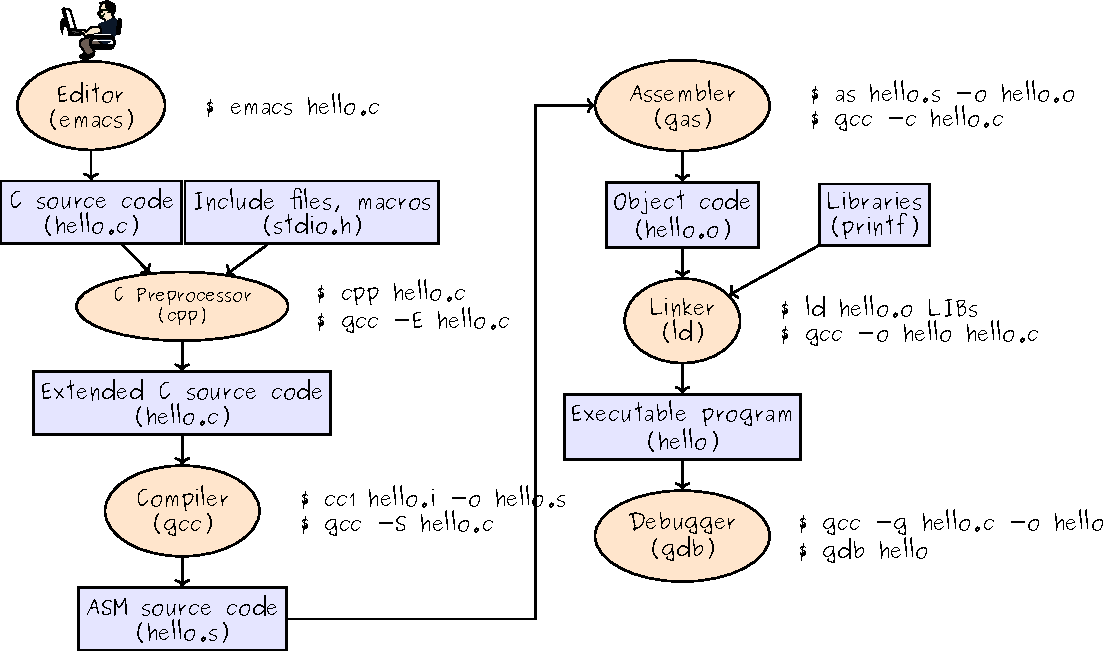
\includegraphics[width=\textwidth]{toolchain2} }%
  \mode<article>{ 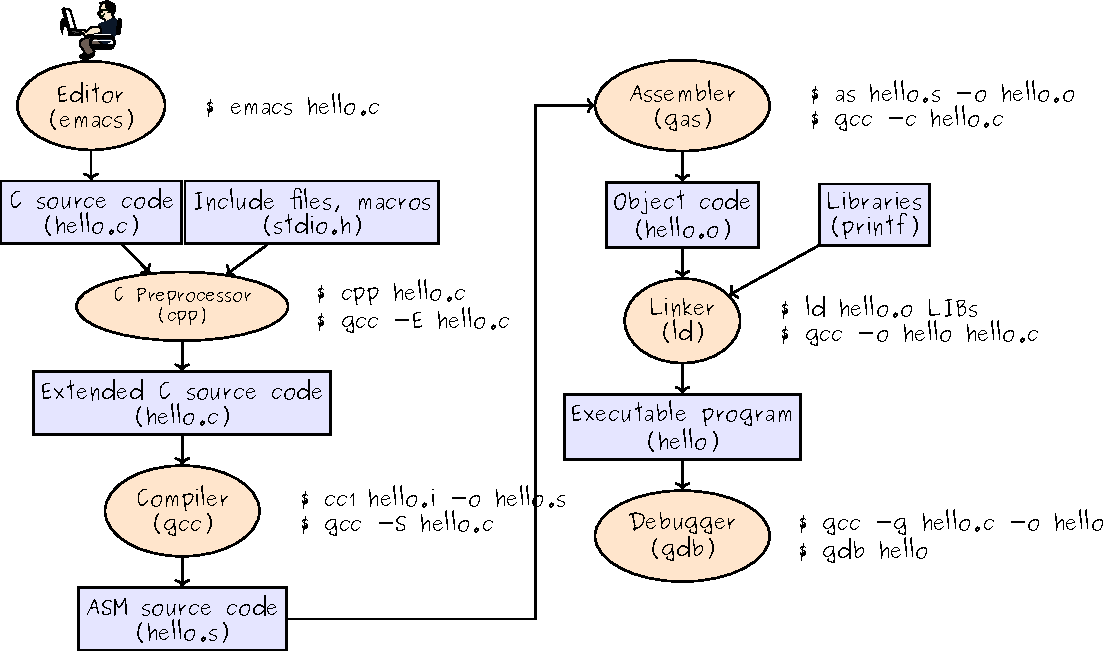
\includegraphics[width=.6\textwidth]{toolchain2} }
\end{center}
\end{frame}

\begin{description}
\item[Source code] written by programmer in high-level language, in our case in
  \texttt{C}. We write c source code with a \emph{text editor}, such as \texttt{emacs},
  \texttt{vim}, etc.
\item[Preprocessing] is the first pass of any C compilation. It processes
  \texttt{include-files}, \texttt{conditional compilation instructions} and
  \texttt{macros}.
  \begin{description}
  \item[cpp] The GNU C preprocessor
    \begin{itemize}
    \item[\$] \texttt{gcc -E hello.c}
    \end{itemize}
  \end{description}
\item[{Compilation}] is the second pass. It takes the output of the preprocessor, and the
  \texttt{source code}, and generates \texttt{assembly source code}.
  \begin{description}
  \item[gcc/g++] GNU C/C++ compiler
    \begin{itemize}
    \item[\$] \texttt{gcc -S hello.c}
    \end{itemize}
  \end{description}
\item[Assembly] is the third stage of compilation. It takes the assembly source code and
  produces an assembly listing with offsets. The assembler output is stored in an
  \texttt{object file}.
  \begin{description}
  \item[as] the portable GNU assembler
    \begin{itemize}
    \item[\$] \texttt{gcc -c hello.c}
    \end{itemize}
  \end{description}
\item[Linking] is the final stage of compilation. It combines object code with predefined
  routines from \texttt{libraries} and produces the \texttt{executable program}.
  \begin{description}
  \item[ld] The GNU linker
    \begin{itemize}
    \item[\$] \texttt{gcc hello.c -lm}
    \end{itemize}
  \end{description}
\item[{Wrapper}] The whole compilation process is usually not done `by hand', but using a
  \texttt{wrapper} program that combines the functions of preprocessor(cpp),
  compiler(gcc/g++), assembler(as) and linker(ld).
  \begin{itemize}
  \item[\$] \texttt{gcc -Wall hello.c -lm -o hello}
  \end{itemize}
\end{description}

See also: \href{http://www.tenouk.com/ModuleW.html}{COMPILER, ASSEMBLER, LINKER AND LOADER:
A BRIEF STORY}.\footnote{\url{http://www.tenouk.com/ModuleW.html}}

\section{Basic Building Blocks of C}

\begin{frame}[fragile]{Basic Building Blocks of C}
  \begin{block}{Data}
    different \alert{types} of \alert{variables}. Examples:
    \begin{multicols}{3}
      \begin{itemize}
      \item[int] v1;
      \item[int] v2;
      \item[int] sum;
      \item[char] c;
      \item[double] i;
      \end{itemize}
    \end{multicols}
  \end{block}
  \begin{block}{Instructions}
    tell the computer what to do with the data.
    \begin{multicols}{2}
      \begin{itemize}
      \item Operators ($+, -, \times{}, \div{}, ...$)
      \item Assignment statement ($=$)
      \item Control statement (\mintinline{c}{if else; for; while; ...})
      \end{itemize}
    \end{multicols}
  \end{block}
  Examples:
  \begin{center}
\begin{ccode}
v1=5; v2=6;
sum = v1 + v2;
if (sum != 11) printf("Wrong!\n");
\end{ccode}    
  \end{center}
\end{frame}

\begin{frame}[fragile=singleslide]
  \begin{block}{Operators for shortcuts}
    \begin{center}{\ttfamily
      \begin{tabular}{llll}
        x++; & x += 2; & x *= 4; & x \%= 6;\\
        x--; & x -= 3; & x /= 5; & \\
      \end{tabular}}
    \end{center}
  \end{block}
\begin{ccode}
n = 5;
npp = n++; /* npp is 5 */
ppn = ++n; /* ppn is 6 */
\end{ccode}
  \begin{block}{The result (11 or 13) actually depends on the compiler}
    {\ttfamily
    \begin{enumerate}
    \item int i=1;
    \item i = (i++ * 5) + (i++ * 3);\quad\tikzmark{nogood}
    \end{enumerate}
    \begin{center}
      \begin{tabular}{l}
        \\
        \textcolor{red}{1}\tikzmark{a1} * 5 + \tikzmark{a2}\textcolor{red}{2} * 3 = 11\\[4ex]
        \textcolor{red}{2}\tikzmark{b2} * 5 + \tikzmark{b1}\textcolor{red}{1} * 3 = 13
      \end{tabular}
    \end{center}}
    \begin{tikzpicture}[remember picture,overlay]
      \node at (pic cs:nogood) [scale=1.2,red,opacity=.4,rotate=25] {{\humor No good}};
      \draw[overlay, ->, blue] ($(pic cs:a1)+(0,7pt)$) to [bend left=25] node [auto,inner sep=1pt] {++} ($(pic cs:a2)+(0,7pt)$);
      \draw[overlay, ->, blue] ($(pic cs:b1)+(0,7pt)$) to [bend right=25] node
      [auto,swap,inner sep=1pt] {++} ($(pic cs:b2)+(0,7pt)$);
    \end{tikzpicture}
  \end{block}
\end{frame}

\begin{frame}[fragile]{Functions}
    \begin{minipage}{.45\linewidth}
\begin{ccode}
int plus(int x, int y){
  int sum = x + y;
  return sum;
}
\end{ccode}      
    \end{minipage}\quad
    \begin{minipage}{.45\linewidth}
\begin{ccode}      
int main(void){
  int v1=5, v2=6;
  int sum = plus(5,6);
  return 0;
}
\end{ccode}
    \end{minipage}
    \begin{block}{Recursion --- A function calls itself}
      \begin{minipage}[t]{.5\linewidth}
\begin{ccode}
int factorial(int n){
  if (n == 0) return 1;
  return n*factorial(n-1);
}
\end{ccode}
      \end{minipage}\quad
      \begin{minipage}[t]{.45\linewidth}
\begin{ccode}
int main(void){
  return factorial(5);
}
\end{ccode}
      \end{minipage}
    \end{block}
\end{frame}

\begin{frame}{Files}{Several files can be compiled together into a single executable}
  \begin{block}{hello2.c}
    \begin{center}
      \mode<beamer>{ \includegraphics[width=\textwidth]{hello2-c} }%
      \mode<article>{ \includegraphics[width=.6\textwidth]{hello2-c} }
    \end{center}
  \end{block}
  \begin{minipage}[b]{.4\linewidth}
    \begin{block}{hello.h}
      \mode<beamer>{ 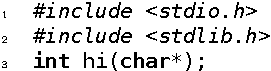
\includegraphics[width=\textwidth]{hello-h} }%
      \mode<article>{ 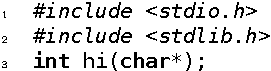
\includegraphics[width=.6\textwidth]{hello-h} }
    \end{block}
  \end{minipage}\quad
  \begin{minipage}[b]{.55\linewidth}
    \begin{block}{hi.c}
      \mode<beamer>{ 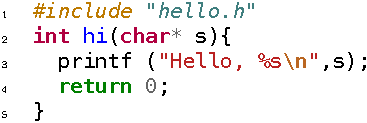
\includegraphics[width=\textwidth]{hi-c} }%
      \mode<article>{ 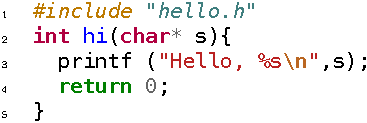
\includegraphics[width=.5\textwidth]{hi-c} }
    \end{block}
  \end{minipage}
\end{frame}

\begin{frame}{Coding Style}
\begin{center}
  \mode<beamer>{ \includegraphics[width=\textwidth]{hello-comments-c} }%
  \mode<article>{ \includegraphics[width=.6\textwidth]{hello-comments-c} }
\end{center}
\end{frame}

\begin{frame}{Variable Types}
  \begin{description}
  \item[Types] char, int, float, double
  \item[Qualifiers] short, long, long long, signed, unsigned
  \end{description}
  \begin{center}{\small
    \begin{tabular}{r|l|l}
      \textbf{Type} & \textbf{Storage size} & \textbf{Value range}\\\hline
      char          & 1 byte        & ${-2^7} \sim {2^7-1}$ or $0 \sim {2^8-1}$\\
      signed char   & 1 byte        & ${-2^7} \sim {2^7-1}$\\
      unsigned char & 1 byte        & $0 \sim {2^8-1}$\\
      int           & 2 or 4 bytes  & ${-2^{15}} \sim {2^{15}-1}$ or ${-2^{31}} \sim {2^{31}-1}$\\
      unsigned int  & 2 or 4 bytes  & $0 \sim {2^{16}-1}$ or $0 \sim {2^{32}-1}$\\
      short         & 2 bytes       & ${-2^{15}} \sim {2^{15}-1}$\\
      unsigned short& 2 bytes       & $0 \sim {2^{16}-1}$\\
      long          & 4 bytes       & ${-2^{31}} \sim {2^{31}-1}$\\
      unsigned long & 4 bytes       & $0 \sim {2^{32}-1}$
    \end{tabular}}
  \end{center}
\end{frame}

\begin{frame}{Integer}
  \begin{block}{Platform dependent}
    \begin{center}
      \mode<beamer>{ 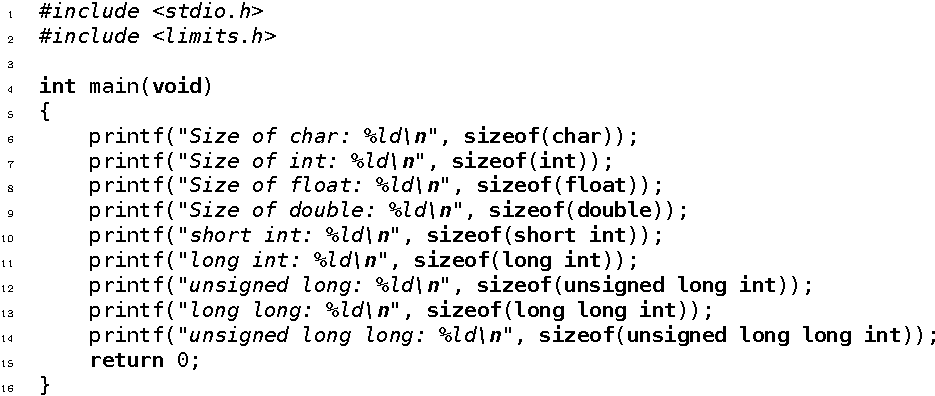
\includegraphics[width=\textwidth]{sizeof-c} }%
      \mode<article>{ 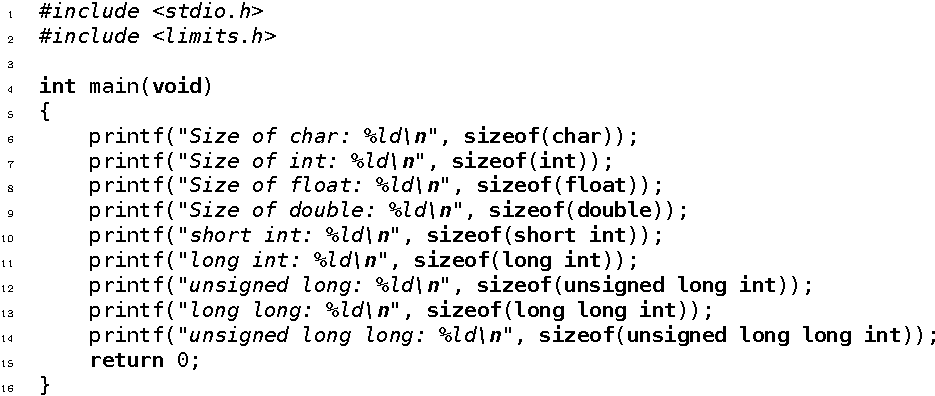
\includegraphics[width=.7\textwidth]{sizeof-c} }
    \end{center}
  \end{block}
\end{frame}

See also: \citetitle[Sec 2.5, \emph{Limits}]{stevens2013advanced}.

\begin{frame}{Floating Point}
  \begin{center}{\small
    \begin{tabular}{r|r|l|r}
Type        &Size &Value range& Precision\\\hline
float       &4 byte       &$1.2\times{}10^{-38}  \sim{}3.4\times{}10^{38}$ & 6 decimal places\\
double      &8 byte       &$2.3\times{}10^{-308} \sim{}1.7\times{}10^{308}$ & 15 decimal places\\
long double &10 byte      &$3.4\times{}10^{-4932}\sim{}1.1\times{}10^{4932}$ & 19 decimal places\\    
    \end{tabular}}
  \end{center}
\begin{center}
  \mode<beamer>{ 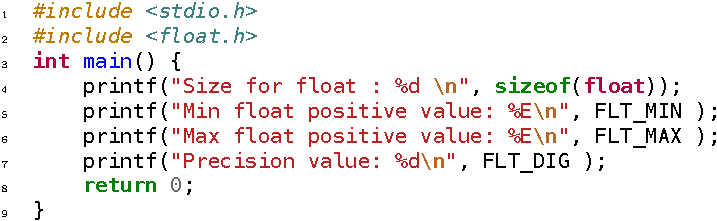
\includegraphics[width=\textwidth]{sizeoffloat-c} }%
  \mode<article>{ 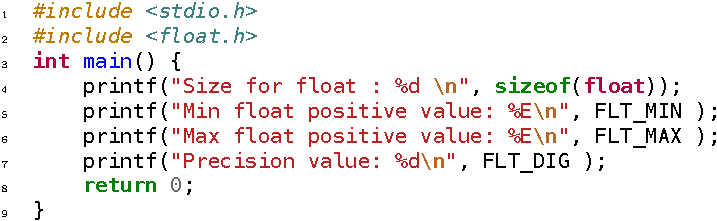
\includegraphics[width=.6\textwidth]{sizeoffloat-c} }
\end{center}
\end{frame}

See also: \href{https://www.tutorialspoint.com/cprogramming/c_data_types.htm}{C data types}
\footnote{\url{https://www.tutorialspoint.com/cprogramming/c_data_types.htm}}

\begin{frame}[fragile]{Variable Names}
  \mode<article>{\begin{multicols}{2}}
    \begin{itemize}
    \item[\Checked] \mintinline{c}{int num_of_students = 10;}
    \item[\Checked] \mintinline{c}{int numOfStudents = 10;}
    \item[\Checked] \mintinline{c}{int _numOfStudents = 10;}
    \item[\Checked] \mintinline{c}{float pi = 3.14159;}
    \item[\Checked] \mintinline{c}{int sum=0, Sum=0, SUM=0; /* case sensitive*/}
    \item[\RedCross] \mintinline{c}{3rd_entry /* starts with a number */}
    \item[\RedCross] \texttt{all\$done} \mintinline{c}{/* contains a '$'*/}%$
    \item[\RedCross] \mintinline{c}{int /* reserved word */}
    \item[\RedCross] \mintinline{c}{phone number /* has a space */}
    \end{itemize}
  \mode<article>{\end{multicols}}
  \end{frame}

\begin{frame}{Simple Operators}
\begin{center}
  \mode<beamer>{ 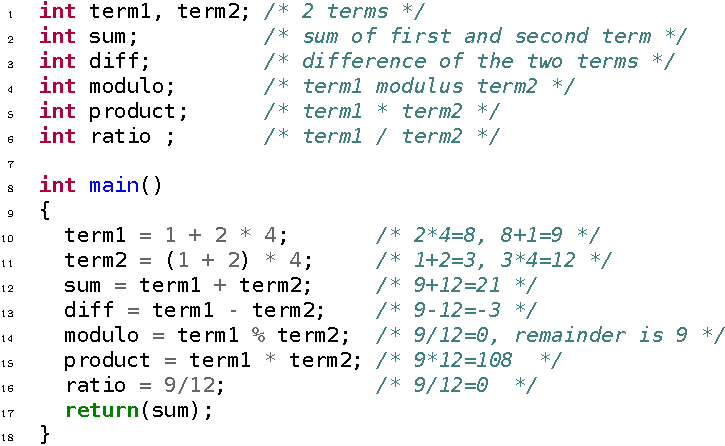
\includegraphics[width=\textwidth]{operators-c} }%
  \mode<article>{ 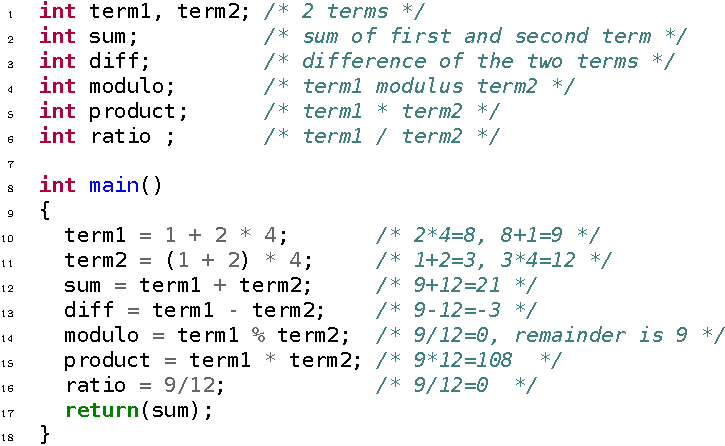
\includegraphics[width=.6\textwidth]{operators-c} }
\end{center}
\end{frame}

\begin{frame}{Floating Point vs. Integer Divide}
  \begin{center}
    \begin{tabular}{lll}\hline
      \textbf{Expression}&\textbf{Result}&\textbf{Result Type}\\\hline
      $19/10$&$1$&integer\\
      $19.0/10$&$1.9$&floating point\\
      $19.0/10.0$&$1.9$&floating point\\\hline
    \end{tabular}
  \end{center}
\end{frame}

\begin{frame}{\texttt{printf(format, expression1, expression2, ...)}}
  \begin{center}{\Large
      \mbox{{\ttfamily
          printf("\%d\tikzmark{a} times \%d\tikzmark{b} is \%d\tikzmark{c} \textbackslash n", \tikzmark{aa}2, \tikzmark{bb}3, \tikzmark{cc}2*3);}}}
  \end{center}
  \begin{tikzpicture}[remember picture,overlay, ->, opacity=.1, ultra thick]
      \draw[red] (pic cs:aa) to [bend left=15] (pic cs:a);
      \draw[blue] (pic cs:bb) to [bend left=25] (pic cs:b);
      \draw[violet] (pic cs:cc) to [bend left=35] (pic cs:c);
    \end{tikzpicture}
\end{frame}

\begin{frame}{\texttt{printf()}}{Escape Characters}
  \begin{center}
    \begin{tabular}{l|l|l}
      \textbf{Character}   &\textbf{Name} &\textbf{Meaning}\\\hline
      \textbackslash b         &backspace       &move cursor one character to the left\\
      \textbackslash f         &form feed       &go to top of new page\\
      \textbackslash n         &newline         &go to the next line\\
      \textbackslash r         &return          &go to beginning of current line\\
      \textbackslash a         &audible alert   &‘beep’\\
      \textbackslash t         &tab             &advance to next tab stop\\
      \textbackslash ’         &apostrophe      &character ’\\
      \textbackslash "         &double quote    &character "\\
      \textbackslash\textbackslash           &backslash       &character\\
      \textbackslash nnn       &                &character number nnn (octal)\\
    \end{tabular}
  \end{center}
\end{frame}

\begin{frame}{\texttt{printf()}}{Format Statements}
  \begin{center}
    \begin{tabular}{l|l|l}
      Conversion   &Argument Type   &Printed as\\\hline
      \%d          &integer         &decimal number\\
      \%f          &float           &[-]m.dddddd (details below)\\
      \%X          &integer         &hex. number using A..F for 10..15\\
      \%c          &char            &single character\\
      \%s          &char *          &print characters from string until '\textbackslash 0'\\
      \%e          &float           &float in exp. form [-]m.dddddde xx\\
      ...&...&...
    \end{tabular}
  \end{center}
  In addition,
  \begin{itemize}
  \item[\%6d] decimal integer, at least 6 characters wide
  \item[\%8.2f] float, at least 8 characters wide, two decimal digits
  \item[\%.10s] first 10 characters of a string
  \item[\$] \texttt{man 3 printf}
  \end{itemize}
\end{frame}

\begin{frame}[fragile=singleslide]{Arrays}
  \begin{block}{}
    \begin{center}
      \mode<beamer>{ 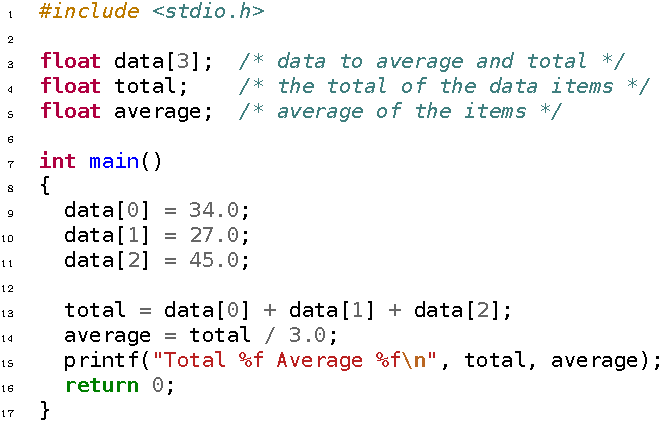
\includegraphics[width=.8\textwidth]{array1-c} }%
      \mode<article>{ 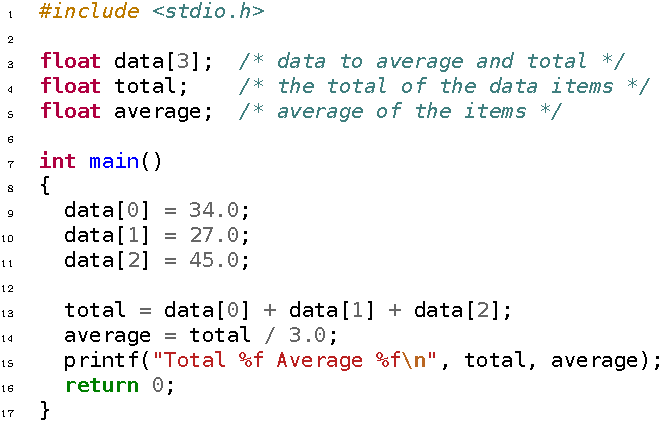
\includegraphics[width=.5\textwidth]{array1-c} }
    \end{center}
  \end{block}
\begin{itemize}
\item[\Checked] \mintinline{c}{int data[3]={10,972,45};}
\item[\Checked] \mintinline{c}{int data[]={10,972,45};}
\item[\Checked] \mintinline{c}{int matrix[2][4]={{1,2,3,4},{10,20,30,40}};}
\end{itemize}
\end{frame}

\begin{frame}[fragile=singleslide]{Strings}
  \begin{description}
  \item[Strings] are \alert{character arrays} with the additional special character ``\verb|\0|''
    (NUL) at the end. E.g.:
    \begin{itemize}
    \item[] \mintinline{c}{char system[] = "Linux";}
    \item[] \begin{tabular}{|p{1ex}|p{1ex}|p{1ex}|p{1ex}|p{1ex}|p{1ex}|} \hline
              L&i&n&u&x&\textbackslash0\\\hline
            \end{tabular}
          \end{itemize}
  \end{description}
  \begin{block}{The most common string functions}
    \begin{center}
      \mode<beamer>{ 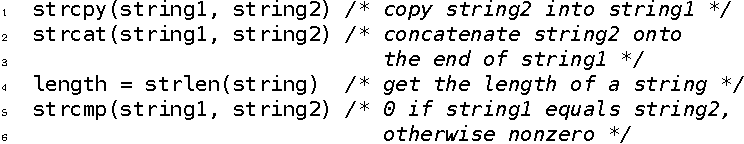
\includegraphics[width=\textwidth]{string-funcs-c} }%
      \mode<article>{ 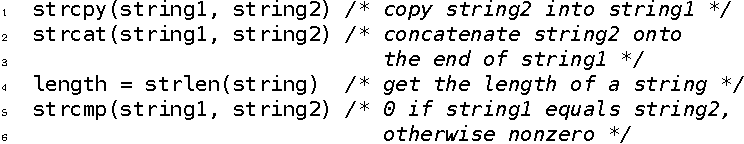
\includegraphics[width=.6\textwidth]{string-funcs-c} }
    \end{center}
  \end{block}
\end{frame}

\begin{frame}
  \begin{block}{Example}
    \begin{center}
      \mode<beamer>{ 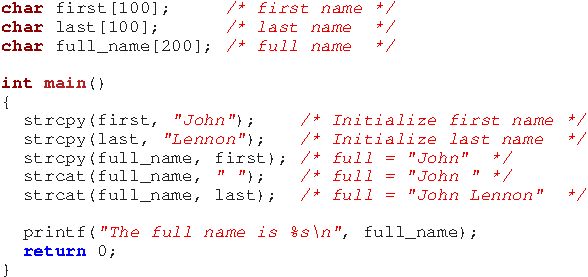
\includegraphics[width=\textwidth]{strcat-c} }%
      \mode<article>{ 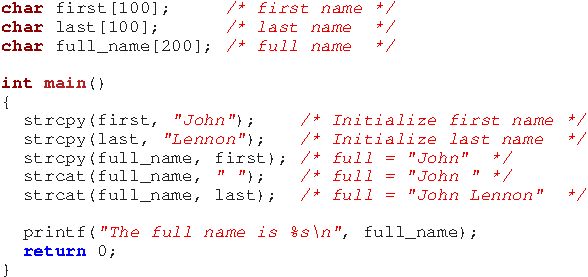
\includegraphics[width=.6\textwidth]{strcat-c} }
    \end{center}
  \end{block}
\end{frame}

\begin{frame}[fragile=singleslide]{fgets()}{Reading in strings from keyboard}
  \mintinline{c}{char *fgets(char *s, int size, FILE *stream);}
  \begin{block}{Example}
    \begin{center}
      \mode<beamer>{ 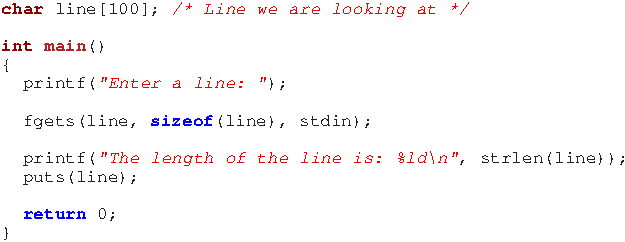
\includegraphics[width=\textwidth]{fgets1-c} }%
      \mode<article>{ 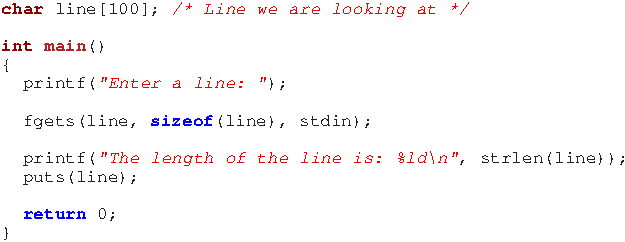
\includegraphics[width=.6\textwidth]{fgets1-c} }
    \end{center}
  \end{block}
  \begin{itemize}
  \item[\$] \texttt{man 3 fgets}
  \end{itemize}
\end{frame}

\begin{frame}
  \begin{block}{Example}
    \begin{center}
      \mode<beamer>{ \includegraphics[width=.6\textwidth]{fgets2-c} }%
      \mode<article>{ \includegraphics[width=.4\textwidth]{fgets2-c} }
    \end{center}
  \end{block}
\end{frame}

\begin{verbatim}
Output of fgets - Example 2:
kaiser@npl03:˜/oreilly/pracc/full1> full1
Enter first name: John
Enter last name: Lennon
The name is John
 Lennon

What happened ? Why is the last name in a new line ?

     The fgets command gets the entire line, including the
     end-of-line. For example, "John" gets stored as
     {’J’,’o’,’h’,’n’,’ n’,’ 0’}.
     This can be fixed by using the statement
     first[strlen(first)-1] = ’ 0’;
     which replaces the end-of-line with an end-of-string character
     and so end the string earlier.
\end{verbatim}

\begin{frame}[fragile=singleslide]{scanf()}{Reading in formatted input from stdin}
  \mintinline{c}{int scanf(const char *format, ...);}
  \begin{block}{Example}
    \begin{center}
      \mode<beamer>{ \includegraphics[width=.7\textwidth]{scanf-c} }%
      \mode<article>{ \includegraphics[width=.5\textwidth]{scanf-c} }
    \end{center}
  \end{block}
\end{frame}

\begin{frame}{if ... else ...}
\begin{center}
  \mode<beamer>{ \includegraphics[width=.8\textwidth]{if1-c} }%
  \mode<article>{ \includegraphics[width=.6\textwidth]{if1-c} }
\end{center}
\end{frame}

\begin{frame}{Relational Operators}
  \begin{multicols}{2}
    \begin{itemize}
    \item[<] less than
    \item[<=] less than or equal
    \item[==] equal
    \item[>] greater than
    \item[>=] greater or equal than
    \item[!=] not equal
    \end{itemize}
  \end{multicols}
\end{frame}

\begin{frame}{Loops}{while}
  \begin{center}
    \mode<beamer>{ \includegraphics[width=.7\textwidth]{while1-c} }%
    \mode<article>{ \includegraphics[width=.3\textwidth]{while1-c} }
  \end{center}
\end{frame}

\begin{frame}{Loops}{for}
  \begin{center}
    \mode<beamer>{ \includegraphics[width=.7\textwidth]{for1-c} }%
    \mode<article>{ \includegraphics[width=.3\textwidth]{for1-c} }
  \end{center}
\end{frame}

\begin{frame}{Loop Control Statements}{break}
  \begin{center}
    \mode<beamer>{ \includegraphics[width=.7\textwidth]{break-c} }%
    \mode<article>{ \includegraphics[width=.3\textwidth]{break-c} }
  \end{center}
\end{frame}

\begin{frame}{Loop Control Statements}{continue}
\begin{center}
  \mode<beamer>{ 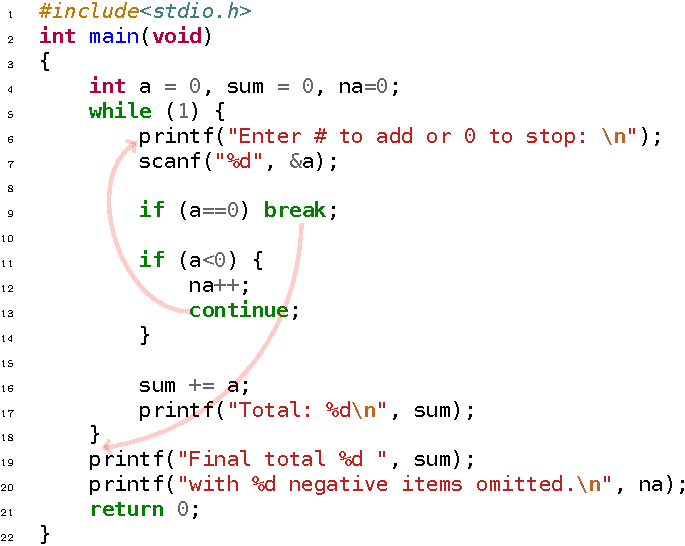
\includegraphics[width=.8\textwidth]{continue-anno} }%
  \mode<article>{ 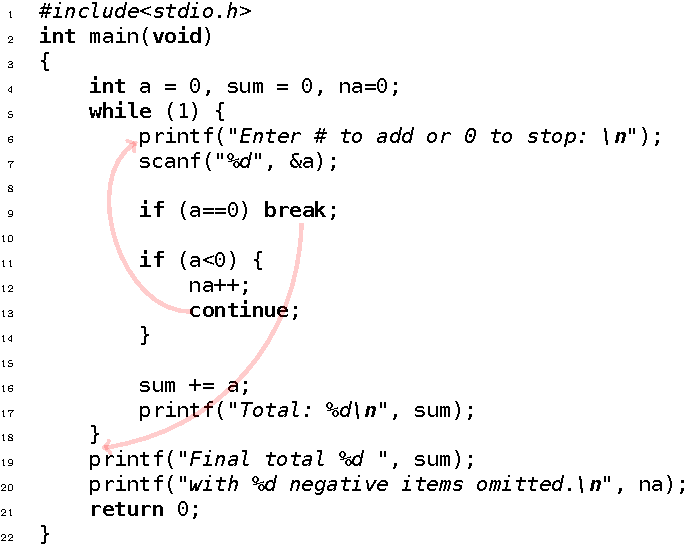
\includegraphics[width=.6\textwidth]{continue-anno-bw} }
\end{center}
\end{frame}

\begin{frame}{switch}
  \begin{center}
    \mode<beamer>{ 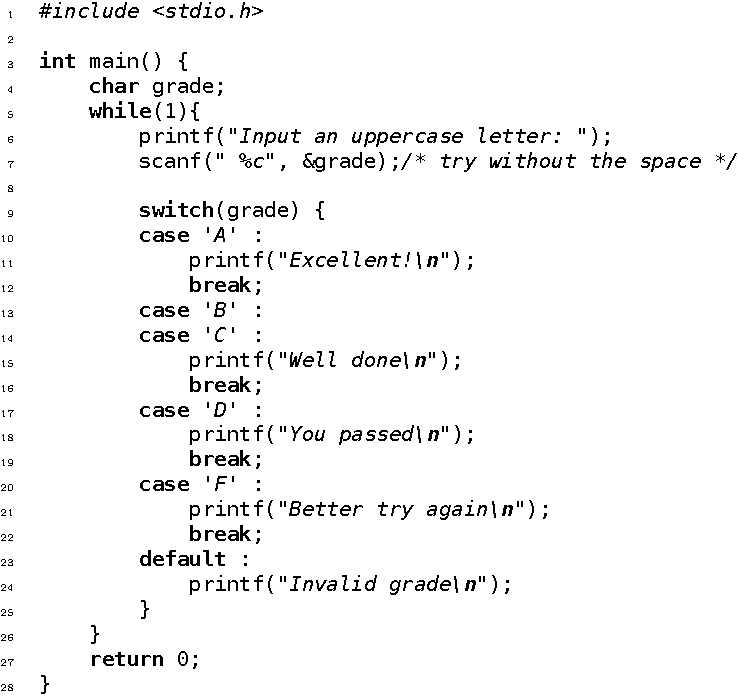
\includegraphics[width=.7\textwidth]{switch1-c} }%
    \mode<article>{ 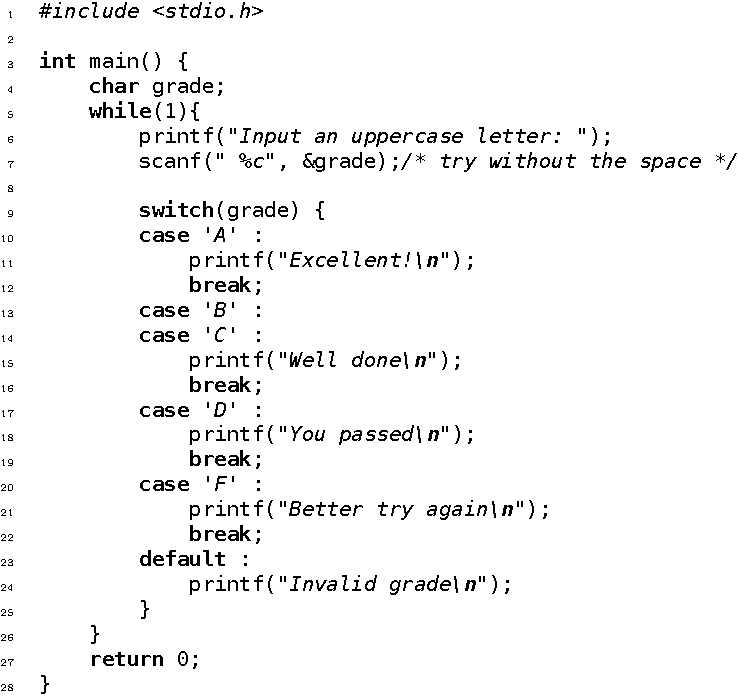
\includegraphics[width=.6\textwidth]{switch1-c} }
  \end{center}
\end{frame}

\begin{frame}
\begin{center}
  \mode<beamer>{ 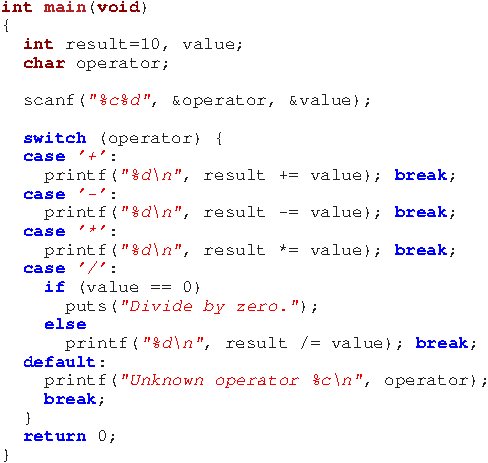
\includegraphics[width=.8\textwidth]{switch2-c} }%
  \mode<article>{ 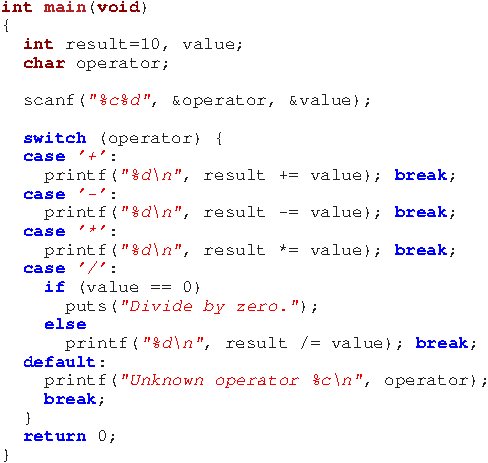
\includegraphics[width=.5\textwidth]{switch2-c} }
\end{center}
\end{frame}

\section{The make Utility}

\begin{frame}{make}
  To compile a single C program:
  \begin{itemize}
  \item[\$] \texttt{gcc hello.c -o hello} \tikz \node [opacity=.4,red,scale=3,inner
    sep=0pt,label={[below=2.5ex,right]{\tiny OK. But...}}] {\Checked};%\textcolor{red}{{\scriptsize OK. But...}}
  \end{itemize}
  \begin{block}{What if you have a large project with 1000+ \texttt{.c} files?}
    \begin{center}
      \mode<beamer>{ 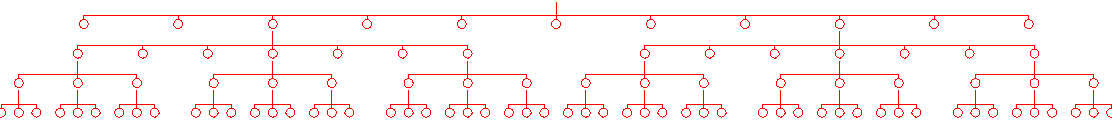
\includegraphics[width=\textwidth]{tree} }%
      \mode<article>{ 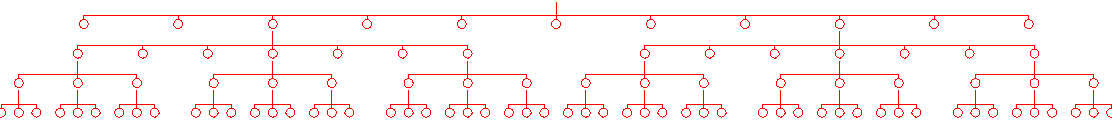
\includegraphics[width=.5\textwidth]{tree} }
    \end{center}
    \begin{description}
    \item[Linux 4.9 source tree:] 3799 directories, 55877 files
    \end{description}
  \end{block}
  \begin{description}
  \item[make:] help you maintain your programs.
  \end{description}
\end{frame}

\begin{frame}{Makefile}
  \begin{block}{}
      \mode<beamer>{ 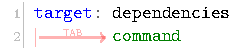
\includegraphics[width=.5\textwidth]{mktab1} }%
      \mode<article>{ 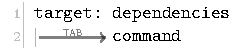
\includegraphics[width=.3\textwidth]{mktab1-bw} }
  \end{block}
  \begin{block}{Example}
      \mode<beamer>{ \includegraphics[width=.6\textwidth]{mktab2} }%
      \mode<article>{ \includegraphics[width=.4\textwidth]{mktab2-bw} }
  \end{block}
  \begin{itemize}
  \item[\$] \texttt{info make makefiles}
  \end{itemize}
\end{frame}

\begin{frame}{Makefile}
  \begin{minipage}{.75\linewidth}
    \mode<beamer>{ \includegraphics[width=\textwidth]{Makefile2-mk} }%
    \mode<article>{ \includegraphics[width=\textwidth]{Makefile2-mk} }
  \end{minipage}
  \begin{minipage}{.2\linewidth}
    \includegraphics[width=\textwidth]{make-dir-tree}
  \end{minipage}
\end{frame}

\section{C Concepts}

\begin{frame}[fragile]{The \texttt{\#include} Instruction}
  \begin{center}
    \includegraphics[scale=1.5]{include-c}\tikzmark{inc}
  \end{center}
\begin{description}
\item[Header files:] for keeping \emph{definitions} and \emph{function prototypes}. E.g.
  \begin{itemize}
  \item \mintinline{c}{#define SQR(x) ((x) * (x))}
  \item \mintinline{c}{ssize_t read(int fildes, void *buf, size_t nbyte);}
  \end{itemize}
\item[Stan\tikzmark{std}dard header files:] define data structures, macros, and function
  prototypes used by library routines, e.g. \texttt{printf()}.
  \begin{itemize}
  \item[\$] \texttt{ls /usr/include}
  \end{itemize}
\item[Loc\tikzmark{local}al include files:] self-defined data structures, macros, and
  function prototypes.
\end{description}
\begin{itemize}
\item[\$] \texttt{gcc -E hello.c}
\end{itemize}
\begin{tikzpicture}[remember picture,overlay,->,blue,ultra thick,opacity=.1]
  \draw ($(pic cs:std)+(0,1ex)$) to[bend left=25] ($(pic cs:inc)+(-2.8,.8)$);
  \draw ($(pic cs:local)+(0,1ex)$) to[bend left=20] ($(pic cs:inc)+(-2.8,.2)$);
\end{tikzpicture}
\end{frame}

\begin{frame}{The \texttt{\#define} Instruction}
  \begin{block}{Always put \alert{\{ \}} around all multi-statement macros!}
    \begin{center}
      \mode<beamer>{
        \includegraphics[width=.8\textwidth]{die-wrong-c}\tikzmark{die-wrong}
        \begin{tikzpicture}[remember picture,overlay,opacity=.3]
          \node (wrong) [scale=5] at ($(pic cs:die-wrong)+(0,3)$) {\RedCross};
        \end{tikzpicture}
      }%
      \mode<article>{
        \includegraphics[width=.4\textwidth]{die-wrong-c}\tikzmark{die-wronga}
        \begin{tikzpicture}[remember picture,overlay,opacity=.3]
          \node (wrong) [scale=5] at ($(pic cs:die-wronga)+(0,2)$) {\RedCross};
        \end{tikzpicture}
      }
    \end{center}
  \end{block}
  \begin{block}{}
    \begin{center}
      \mode<beamer>{ \includegraphics[width=.8\textwidth]{die-right-c}\tikzmark{die-right} }%
      \mode<article>{ \includegraphics[width=.4\textwidth]{die-right-c}\tikzmark{die-right} }
    \end{center}
  \end{block}
  \begin{description}
  \item[Why?] \texttt{gcc -E}
  \end{description}
  \begin{tikzpicture}[remember picture,overlay,opacity=.3]
    \node (right) [scale=5,green] at (pic cs:die-right) {\Checked};
  \end{tikzpicture}
\end{frame}

\begin{frame}[fragile=singleslide]
  \begin{block}{Always put \alert{( )} around the parameters of a macro!}
    \begin{center}
      \mode<beamer>{
        \includegraphics[width=\textwidth]{sqr-wrong-c}\tikzmark{sqr-wrong}
        \begin{tikzpicture}[remember picture,overlay,opacity=.3]
          \node [scale=5] at ($(pic cs:sqr-wrong)+(-6,4.5)$) {\RedCross};
        \end{tikzpicture}
      }%
      \mode<article>{
        \includegraphics[width=.5\textwidth]{sqr-wrong-c}\tikzmark{sqr-wronga}
        \begin{tikzpicture}[remember picture,overlay,opacity=.3]
          \node [scale=5] at ($(pic cs:sqr-wronga)+(-4,3.2)$) {\RedCross};
        \end{tikzpicture}
      }
    \end{center}
  \end{block}
  \begin{itemize}
  \item[\Checked] \mintinline{c}{#define SQR(x) ((x) * (x))}
  \item[\$] \texttt{gcc -E}
  \end{itemize}
\end{frame}

\begin{frame}{Bitwise Operations}
  \begin{center}
    \mode<beamer>{ \includegraphics[width=\textwidth]{bitwise-c} }%
    \mode<article>{ \includegraphics[width=.5\textwidth]{bitwise-c} }
  \end{center}
\end{frame}

\begin{frame}{Pointers}
  \begin{center}
    \mode<beamer>{ \includegraphics[width=.9\textwidth]{ptr1-code-c} }%
    \mode<article>{ \includegraphics[width=.6\textwidth]{ptr1-code-c} }
  \end{center}
  \begin{center}
    \mode<beamer>{ \includegraphics[width=\textwidth]{ptr1} }%
    \mode<article>{ \includegraphics[width=.6\textwidth]{ptr1} }
  \end{center}
\end{frame}

\begin{frame}{Pointer Operators}
  \begin{itemize}
  \item[\&] returns the \alert{address} of a thing
  \item[{\dejavu ✶}] return the \alert{object (thing)} to which a pointer points at
  \end{itemize}
  \begin{block}{\texttt{int thing; int *thing\_ptr;}}
    \begin{center}
      \begin{tabular}{r|l}
        \textbf{C Code}&\textbf{Description}\\\hline
        \texttt{thing}& the variable named `thing'\\
        \texttt{\&thing}& address of `thing' (a pointer)\\
        \texttt{*thing}& \RedCross{}\\
        \texttt{thing\_ptr}& pointer to an int\\
        \texttt{*thing\_ptr}& the int variable at the address \texttt{thing\_ptr} points
                              to\\
        \texttt{\&thing\_ptr}& odd, a pointer to a pointer
      \end{tabular}
    \end{center}
  \end{block}
\end{frame}

\begin{frame}
  \begin{block}{Example}
    \begin{center}
      \mode<beamer>{ \includegraphics[width=.9\textwidth]{ptr2-code-c} }%
      \mode<article>{ \includegraphics[width=.6\textwidth]{ptr2-code-c} }
    \end{center}
  \end{block}
  \begin{center}
    \mode<beamer>{ \includegraphics[width=.8\textwidth]{ptr2} }%
    \mode<article>{ \includegraphics[width=.4\textwidth]{ptr2} }
  \end{center}
\end{frame}

\begin{frame}
  \begin{block}{Invalid operation}
    \begin{center}
      \mode<beamer>{ \includegraphics[width=.7\textwidth]{ptr2-wrong1-c} }%
      \mode<article>{ \includegraphics[width=.5\textwidth]{ptr2-wrong1-c} }
    \end{center}
    \mode<article>{
      This is trying to treat the value of \texttt{i} as an memory address. But the memory
      address \texttt{5} is not accessible by this program.
    }
  \end{block}
  \begin{block}{Invalid memory access}
    \begin{center}
      \mode<beamer>{ \includegraphics[width=.8\textwidth]{ptr2-wrong2-c} }%
      \mode<article>{ \includegraphics[width=.6\textwidth]{ptr2-wrong2-c} }
    \end{center}
    \mode<article>{
      This is trying to treat the value of \texttt{p} as an memory address. But the memory
      address \texttt{5} is not accessible by this program.
    }
  \end{block}
\end{frame}

\begin{frame}{Call by Value}
  \begin{center}
    \mode<beamer>{
      \includegraphics[width=.6\textwidth]{ptr4-wrong-c}\tikzmark{ptr4wrong}
      \pause
      \begin{tikzpicture}[remember picture,overlay]
        \node at ($(pic cs:ptr4wrong)+(1,2)$) [opacity=.4,scale=7] {\RedCross};
      \end{tikzpicture}}%    
    \mode<article>{
      \includegraphics[width=.3\textwidth]{ptr4-wrong-c}\tikzmark{ptr4wronga}
      \begin{tikzpicture}[remember picture,overlay]
        \node at ($(pic cs:ptr4wronga)+(1,2)$) [opacity=.4,scale=7] {\RedCross};
      \end{tikzpicture}}    
  \end{center}
  \begin{description}
  \item[Call by value:] only the \alert{value} of `\texttt{count}' is handed to the
    function \texttt{inc\_count()}
  \end{description}
\end{frame}

\begin{frame}
  \begin{block}{Solution 1: return}
    \begin{center}
      \mode<beamer>{
        \includegraphics[width=.7\textwidth]{ptr4-ok-c}
        \begin{tikzpicture}[remember picture,overlay]
          \node at ($(pic cs:ptr4ok)+(0,2)$) [opacity=.4,scale=10,red] {\Checked};
        \end{tikzpicture}}%
      \mode<article>{
        \includegraphics[width=.4\textwidth]{ptr4-ok-c}\tikzmark{ptr4oka}
        \begin{tikzpicture}[remember picture,overlay]
          \node at ($(pic cs:ptr4oka)+(0,2)$) [opacity=.4,scale=10,red] {\Checked};
        \end{tikzpicture}
        \begin{enumerate}
        \item read the \emph{value} of \texttt{count}, and pass it to \texttt{inc\_count()};
        \item \texttt{inc\_count()} uses the \emph{value} of \texttt{count} to do the
          calculations;
        \item return the result to \texttt{main()}.
        \end{enumerate}
      }
    \end{center}
  \end{block}
    
\end{frame}

\begin{frame}{Pointers as Function Arguments}
  \begin{block}{Solution 2: Call by reference}
    \begin{center}
      \mode<beamer>{
        \includegraphics[width=.6\textwidth]{ptr4-c}
        \begin{tikzpicture}[remember picture,overlay]
          \node at ($(pic cs:ptr4)+(0,2)$) [opacity=.4,scale=10,red] {\Checked};
        \end{tikzpicture}}%
      \mode<article>{
        \includegraphics[width=.3\textwidth]{ptr4-c}\tikzmark{ptr4a}
        \begin{tikzpicture}[remember picture,overlay]
          \node at ($(pic cs:ptr4a)+(0,2)$) [opacity=.4,scale=10,red] {\Checked};
        \end{tikzpicture}
        \begin{enumerate}
        \item pass the address of \texttt{count} to \texttt{inc\_count()};
        \item \texttt{inc\_count()} operates directly on \texttt{count}.
        \end{enumerate}
        This is more efficient than solution 1 (Imagining you are operating on a large
        data structure rather than an \texttt{int}). 
      }
    \end{center}
  \end{block}    
\end{frame}

\begin{frame}[fragile]{\texttt{const} Pointers}
\begin{ccode}
const char *a_ptr = "Test";
char *const a_ptr = "Test";
const char *const a_ptr = "Test";
\end{ccode}
  \begin{enumerate}
  \item The da\tikzmark{data1}ta cannot change, but the poin\tikzmark{ptr1}ter can
  \item The point\tikzmark{ptr2}er cannot change, but the \tikzmark{data2}data it points to can
  \item Neither can change
  \end{enumerate}
  \mode<beamer>{
  \begin{tikzpicture}[remember picture,overlay,->,blue,ultra thick, opacity=.1]
  \draw ($(pic cs:data1)+(0,1ex)$) to[bend left=25] ($(current page.center)+(-1.5,1.8)$);
  \draw ($(pic cs:ptr1)+(0,1ex)$) .. controls +(1,1.5) and +(1.5,1.2) .. ($(current page.center)+(-2.3,1.9)$);
  \draw ($(pic cs:data2)+(0,1ex)$) to ($(current page.center)+(-.8,1.3)$);
  \draw ($(pic cs:ptr2)+(0,1ex)$) to ($(current page.center)+(-2.4,1.3)$);
\end{tikzpicture}}
\end{frame}

\section{Pointers and Arrays}

\begin{frame}
  \begin{minipage}[t]{.44\linewidth}
    \includegraphics[width=\textwidth]{array2-c}
  \end{minipage}
  \begin{minipage}[t]{.52\linewidth}
    \includegraphics[width=\textwidth]{array2-2-c}\tikzmark{array2-2}
    \mode<beamer>{
      \begin{tikzpicture}[remember picture,overlay]
        \node at ($(pic cs:array2-2)+(-.68,.91)$) [ellipse,opacity=.4,red,draw,thick,minimum
        width=1cm] {};
      \end{tikzpicture}}
    \mode<article>{
      \begin{tikzpicture}[remember picture,overlay]
        \node at ($(pic cs:array2-2)+(-.9,1.4)$) [ellipse,opacity=.4,red,draw,thick,minimum
        width=1.5cm] {};
      \end{tikzpicture}
      C automatically scales pointer arithmetic so that it works correctly, by
      incrementing/decrementing by the correct number of bytes. For example, at line 11,
      the value of \texttt{pa} is \texttt{1008}, and the value of \texttt{a} is
      \texttt{1000}. But the result of ``\texttt{pa - a}'' is \texttt{2} rather than
      \texttt{8}. This means \texttt{pa} is \emph{two ints} ahead of \texttt{a}.}
  \end{minipage}
  \begin{center}
    \mode<beamer>{ \includegraphics[width=\textwidth]{array2-3} }%
    \mode<article>{ \includegraphics[width=.6\textwidth]{array2-3} }
  \end{center}
\end{frame}

\begin{frame}{Passing Arrays to Functions}
  \begin{block}{}
    When passing an array to a function, C will automatically change the array into a
    pointer.
  \end{block}  
  \begin{minipage}{.47\linewidth}
    \begin{center}
      \mode<beamer>{ \includegraphics[width=\textwidth]{array3-1-c} }%
      \mode<article>{ \includegraphics[width=.6\textwidth]{array3-1-c} }
    \end{center}
  \end{minipage}\hfill
  \begin{minipage}{.47\linewidth}
    \begin{center}
      \mode<beamer>{ \includegraphics[width=\textwidth]{array3-2-c} }%
      \mode<article>{ \includegraphics[width=.6\textwidth]{array3-2-c} }
    \end{center}
  \end{minipage}
\end{frame}

\begin{frame}[fragile]{Arrays of Pointers}
  \begin{center}
    \mode<beamer>{ \includegraphics[width=.7\textwidth]{array4-c} }%
    \mode<article>{ \includegraphics[width=.5\textwidth]{array4-c} }
  \end{center}
\end{frame}

\paragraph*{Once you've declared an array, you can't reassign it. Why?}
[\url{https://stackoverflow.com/questions/17077505/string-pointer-and-array-of-chars-in-c}]

Consider an assignment like

\begin{ccode}
char *my_str = "foo"; // Declare and initialize a char pointer.
my_str = "bar"; // Change its value.
\end{ccode}

The first line declares a char pointer and ``aims'' it at the first letter in \texttt{foo}. Since \texttt{foo} is a string constant, it resides somewhere in memory with all the other constants. When you reassign the pointer, you're assigning a new value to it: the address of \texttt{bar}. But the original string, \texttt{foo}, remains unchanged. You've moved the pointer, but haven't altered the data.

\emph{When you declare an array, however, you aren't declaring a pointer at all. You're reserving a certain amount of memory and giving it a name}. So the line

\begin{ccode}
char c[5] = "data";
\end{ccode}

starts with the string constant \texttt{data}, then allocates 5 new bytes, calls them \texttt{c}, and copies the string into them. You can access the elements of the array exactly as if you'd declared a pointer to them; arrays and pointers are (for most purposes) interchangeable in that way.

\emph{But since arrays are not pointers, you cannot reassign them}. You can't make
\texttt{c} ``point'' anywhere else, because it's not a pointer; it's the name of an area of
memory. For example,

\begin{ccode}
char c[5] = "data";
char b[5] = "beta";
b = c; /* Wrong! 'b[]' cannot be reassigned (pointing to elsewhere). */
\end{ccode}

\begin{frame}[fragile=singleslide]{How not to Use Pointers}
  \begin{block}{Life is complicated enough, don't make it worse}
\begin{ccode}
/* Point to the first element of the array. */
data_ptr = &array[0];

/* Get element #0, data_ptr points to element #1. */
value = *data_ptr++;

/* Get element #2, data_ptr points to element #2. */
value = *++data_ptr;

/* Increment element #2, return its value.
   Leave data_ptr alone. */
value = ++*data_ptr;
\end{ccode}
  \end{block}
  \begin{tikzpicture}[remember picture,overlay]
    \node at ($(current page.center)+(4.5,-2)$) [opacity=.2,red,scale=10] {\bad};
  \end{tikzpicture}  
\end{frame}

\begin{frame}[fragile]
  \begin{block}{Just don't do it}
\begin{ccode}
void copy_string(char *p, char *q)
{
  while (*p++ = *q++);
}
\end{ccode}
  \begin{tikzpicture}[remember picture,overlay]
    \node at ($(current page.center)+(2,-2)$) [opacity=.2,red,scale=20] {\bad};
  \end{tikzpicture}  
  \end{block}
\end{frame}

% https://ocw.mit.edu/courses/electrical-engineering-and-computer-science/6-s096-effective-programming-in-c-and-c-january-iap-2014/lecture-notes/

% https://ocw.mit.edu/courses/electrical-engineering-and-computer-science/6-088-introduction-to-c-memory-management-and-c-object-oriented-programming-january-iap-2010/lecture-notes/

\section{Memory Model}
\begin{frame}{Memory Model}
\begin{center}
  \mode<beamer>{ \includegraphics[width=.7\textwidth]{mem-model} }%
  \mode<article>{ \includegraphics[width=.4\textwidth]{mem-model} }
\end{center}
\end{frame}

\begin{itemize}
\item See also: \citetitle[Sec 0x270 \emph{Memory Segmentation}]{erickson2008hacking}
\item stack setup [linux sys slides]
\item \url{http://www.dirac.org/linux/gdb/02a-Memory_Layout_And_The_Stack.php}
\item gdb (info frame, info args, info locals, ...)
\item \fxnote[inline]{make a good example using both printf() and gdb to show internals of a process}
\end{itemize}

\section{x86 Assembly}

\begin{itemize}
\item \citetitle[Sec 0x253 \emph{Assembly Language}]{erickson2008hacking}
\item \citetitle{jeff16assembly}
\item \citetitle{neveln2000linux}
\end{itemize}

\section{Hacker's Tools}

gdb, objdump, readelf, nm, ...
\begin{itemize}
\item \citetitle{levine2000linkers}
\item \citetitle{salomon1992assemblers}
\end{itemize}

\section{Linux GUI Programming}

\subsection{ncurses}

\subsection{GTK}

\section{APUE}
\subsection{File I/O}
\subsection{Processes and Threads}


% https://denniskubes.com/2012/08/17/basics-of-memory-addresses-in-c/
\end{document}
% (setq-default TeX-master nil)

%%% Local Variables:
%%% mode: latex
%%% TeX-master: "c-b"
%%% End:
